\documentclass[letterpaper]{article}
\usepackage{natbib,alifexi}
\usepackage[utf8]{inputenc}
\usepackage{amsmath}
\usepackage[toc,page]{appendix}
\usepackage[frenchb]{babel}
\usepackage[T1]{fontenc}
\usepackage{placeins, latexsym, amssymb}
\usepackage{comment}
\usepackage{algorithm}
\usepackage{algorithmic}
\usepackage[hidelinks]{hyperref}
\usepackage{verbatim}
\usepackage{listings}

\title{Time stretching en temps réel dans le cadre du live coding}
\author{Abdeselam El-Haman Abdeselam$^{1}$\\
Superviseur : Bernard Fortz
\mbox{}\\\\
$^1$Université Libre de Bruxelles \\
aelhaman@ulb.ac.be}

\setlength{\parskip}{0.8em}

\begin{document}
\maketitle

\begin{abstract}
  Overtone est une libraire en Clojure qui est utilisée pour faire du
  Live Coding (l'art de programmer en \og vif \fg{}). Une des techniques les
  plus utilisées dans le domaine de la musique synthétisée est le
  time-stretching, qui consiste à rallonger ou rétrécir une pièce musicale
  sans changer sa tonalité. Le time-stretching est intéressant dans
  le live-coding lorsqu'on peut modifier les paramétres de celui-ci
  en temps réel. Dans cet article une méthode de time-stretching avec des
  approches différentes sera analysée et utilisée en temps
  réel avec Overtone.

\end{abstract}

\section{Introduction}

  Depuis le débuts de la musique éléctronique, le ``resampling'' de pièces musicales
  (c'est à dire, la manipulation de celles-ci) a un rôle important pour pouvoir manipuler
  des pièces musicales (rajouter des filtres, des envelopes, etc \ldots ).

  Un son est un signal qui est défini par sa durée, sa fréquence et son amplitude. La fréquence
  définit son ``pitch'' ou tonalité. La tonalité d'un son est plus grave si la fréquence est plus
  petite (donc une période plus grande).
  
  La manipulation d'un son dans le temps est utilisée très souvent lors du mixage et DJing.
  Ce genre de manipulations aident à rétrécir ou prolonger cette pièce pour, par exemple, mettre
  un son à la même vitesse que le ``tempo'' d'une chanson.

  Cette manipulation aura comme résultat aussi un effet sécondaire. La prolongation du signal
  provoquera aussi que la fréquence de ce signal soit modifié, et avec ça, un changement
  de tonalité non désiré se produira [\cite{RESAMPLING}].

  \begin{figure}[h]
    \centerline{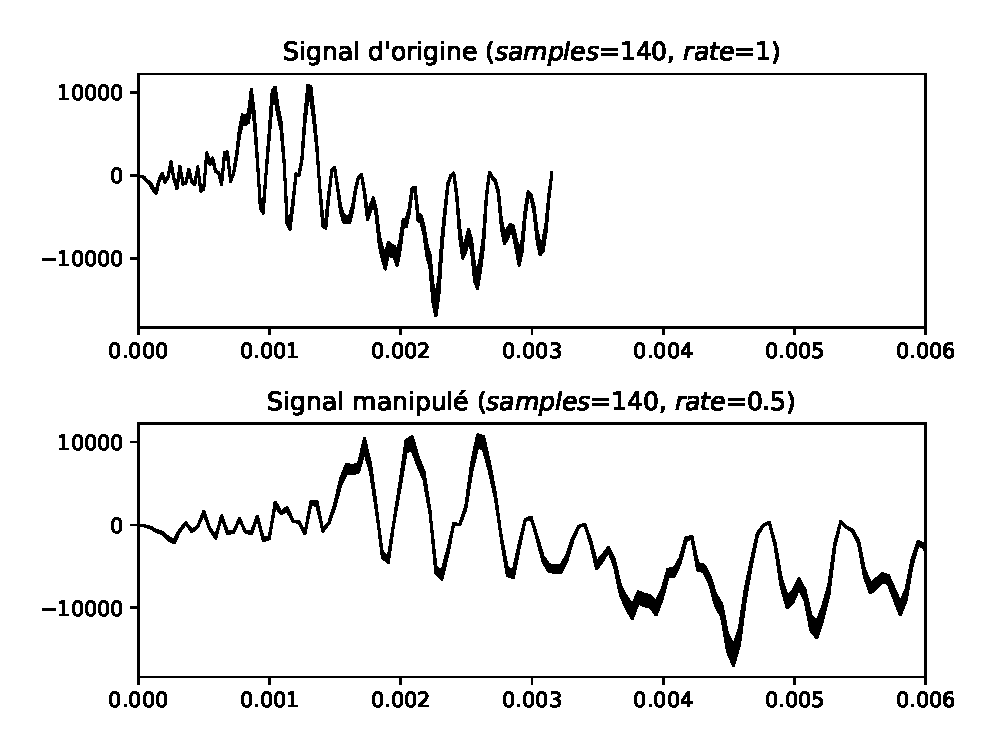
\includegraphics[width=9cm]{res/fig1.eps}}
    \caption{\label{fig:guitar-stretch}Échantillon d'une guitare lu à des vitesses différents}
  \end{figure}
  
  Le time-stretching est une technique pour éradiquer ce problème: changer le tempo d'un
  son sans changer sa tonalité.

  Plusieurs algorithmes existent pour implementer cette technique. Dans cet article l'état de
  l'art du time-stretching sera étudié et plusieurs de ces algorithmes seront
  implémentés pour l'application en temps réel de cette technique sur Overtone, une librairie pour
  qui a été conçue pour le traitement et synthèse de son. 

\section{État de l'art}
\subsection{Méthode OLA}
\paragraph{}En général la méthode utilisée dans les algorithmes TSM se résume en plusieures étapes
distinctes.

\paragraph{Décomposer le signal d'entrée en grains} Le signal d'entrée est décomposé en
\emph{grains} [citer article] d'une taille rélativement petite et fixe. Chacun de ces ces grains sa un décalage \emph{hopsize} $H_{a}$ (hopsize d'analyse). On peut représenter ça tel que:
$$x_m(r) = x(r + mH_{a}) : r \in [-N/2 : N/2 -1]$$
où $x$ est notre signal d'entrée en format discret de taille $L \in \mathbb{Z}_{\geq0}$. $N$ est la
taille du grain $x_m$.

La taille de ces grains doît est généralement d'une taille entre 50ms et 100ms. Ceci est important
pour trouver le \emph{pitch local} dans l'intervale $[mH_{a} - N/2 : mH_{a} + N/2 +1]$. Si l'intervale
est grand, plusieures tonalités apparaissent dans cet intervale, donc ce grain n'est pas représentatif.
\paragraph{Modifier le hopsize} Une fois le signal décomposé, avec l'information de pitch dans chaque grain, on va définir un nouveau hopsize $H_{s}$ qui va servir à récomposer ces grains. Ce $H_{s}$ est défini tel que :

$$H_{s} = \alpha H_{a}$$

Dans lequel $\alpha$ représente le \emph{facteur d'échelle}.
L'effet du TSM est fixé par le \emph{facteur d'échelle}. Pour un effet de rétrécissement:
$$\alpha < 1$$

Au contraire, pour un effet d'élargissement:
$$\alpha > 1$$

\paragraph{Superposition de grains}

Avec $H_{s}$ défini, on peut réconstruire le signal résultat de cette modification, en récomposant
le nouveau signal avec les \emph{grains} avec un décalage de $H_{s}$ au lieu de $H_{a}$. Alors ces
grains sont superposés avec une différence de $H_{s}$ et additionés. C'est à dire:

$$ y(t) = \sum_{m \in \mathbb{Z}} x_{m}(t-mH_{s})$$

où $y(t)$ est le signal de sortie par rapport au temps $t$.
u
\paragraph {Fenêtrage}

Hormis le fait que cette méthode est utilisée comme base des algorithmes qui seront illustrés plus
tard dans ce document, elle crée beaucoup d'\emph{artéfacts} à cause d'un déphasage entre les
grains qui provoque des discontinuités qui se traduit par des sons lourds et courts qui n'étaient pas
dans le signal initial. Ceci est dû à cause d'un déphasage important entre les grains
puisque $H_{s} \neq H_{a}$.

\begin{figure}[h]
    \centerline{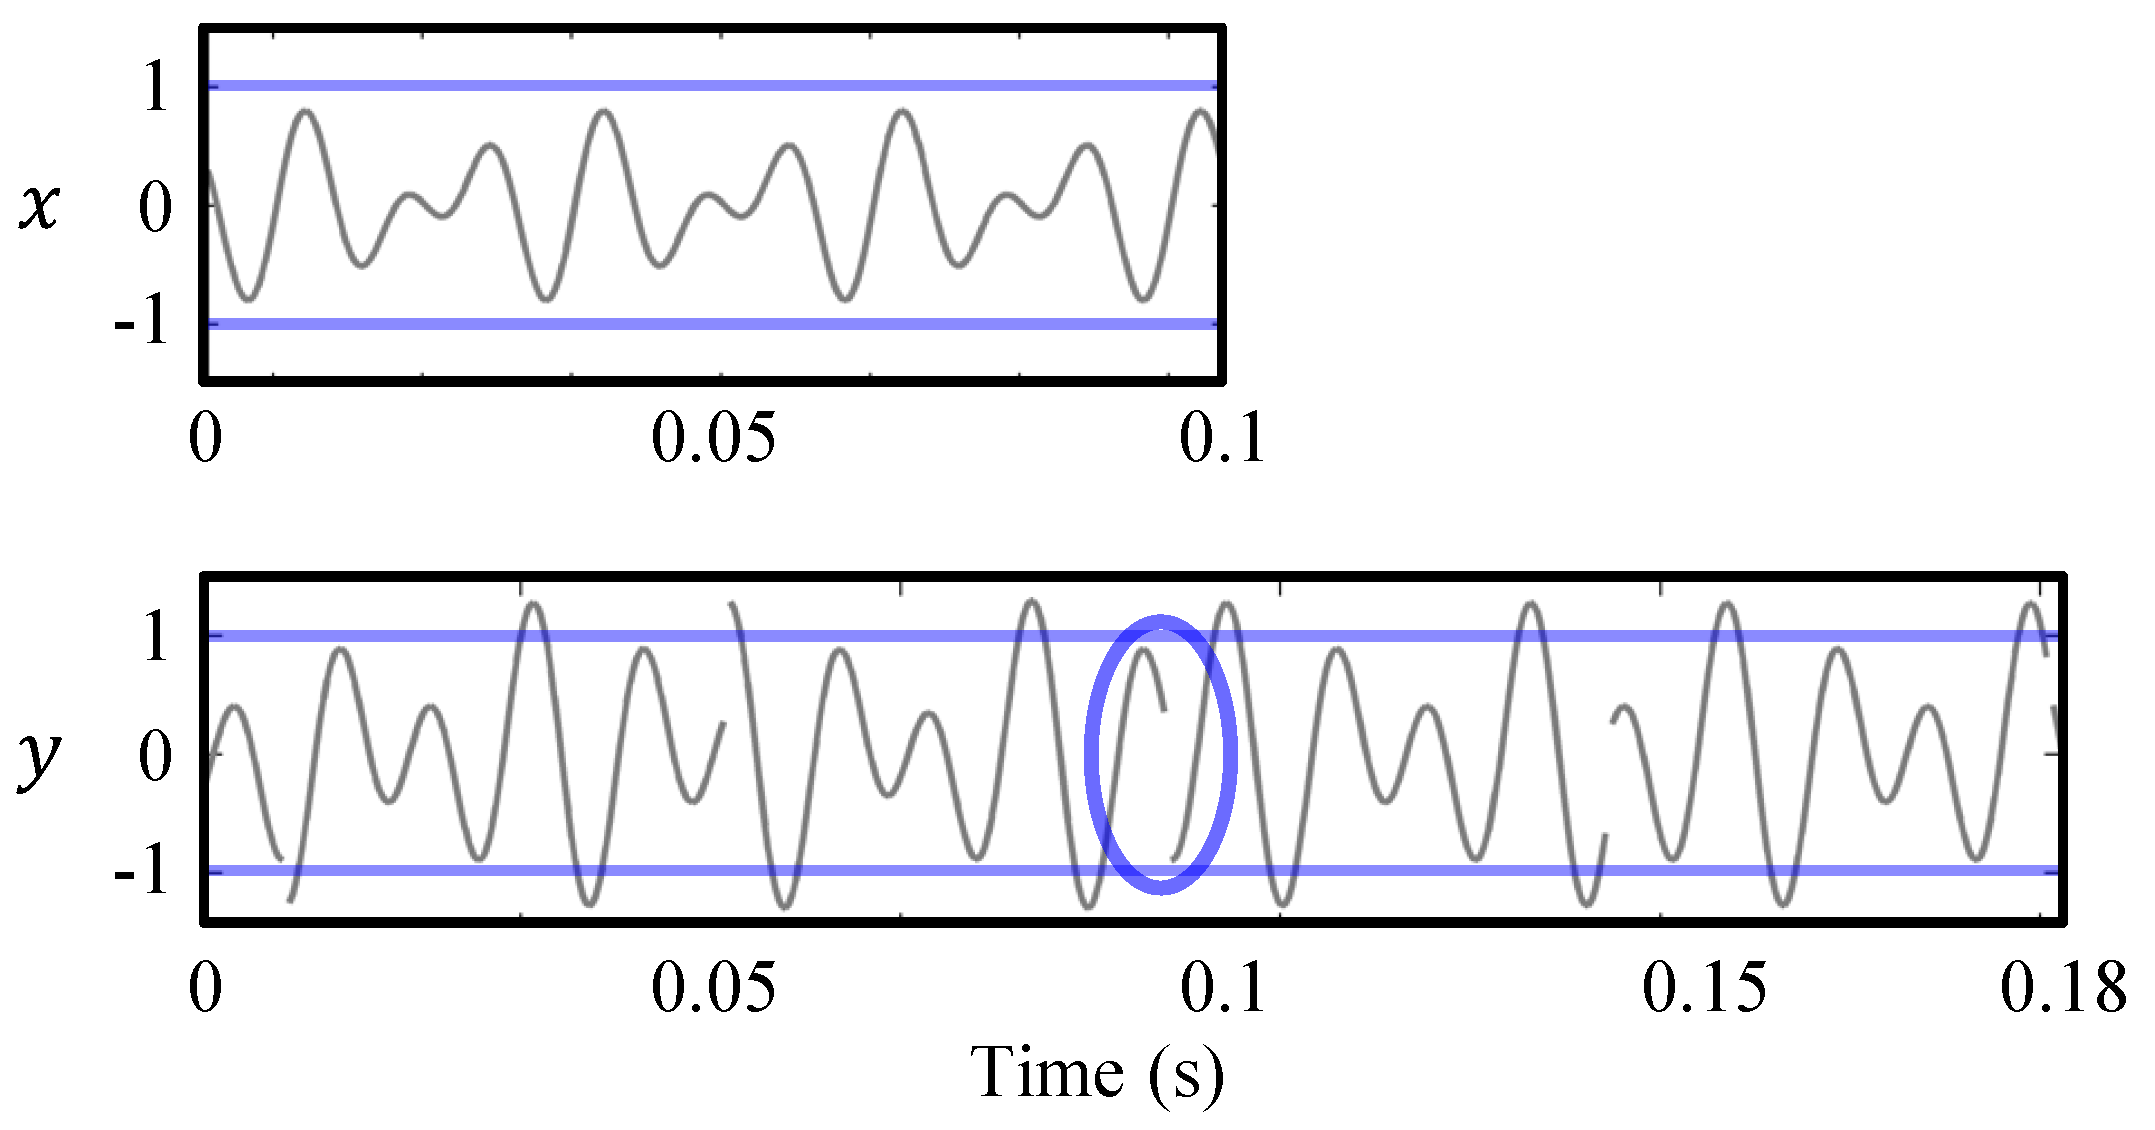
\includegraphics[width=9cm]{res/artifact.png}}
    \caption{\label{fig:artifact}Exemple d'artefact qui se produit quand le même grain d'analyse est
      utilisé pour reconstruire le signal avec le tempo modifié [\cite{TSMreview}]. }
  \end{figure}
  
L'algorithme \emph{OLA} se base sur cette méthode basique et rajoute des fénêtres pour avoir une
fluidité dans la transition d'un grain à un autre. Les grains $x_m$ sont donc appliqués à une fonction
de fênetrage $w$ qui est définie:

$$ w(r) = \frac{1}{2} \bigg(1 - cos \bigg(\frac{2\pi(r + N/2)}{N-1}\bigg) \bigg) $$

Où $w$ est la \emph{fenêtre de Hanning}.

Cette fenêtre a la propriété que

$$ \sum_{n \in \mathbb{Z}} w \bigg( r - n \frac{N}{2} \bigg) = 1 $$

qui rassure la continuité d'amplitude dans le signal résultant. 

\subsection{Méthode WSOLA}

Le problème de la méthode OLA est que, étant le hopsize $H_a$ fixe, chaque séparation entre grains
est le même, peu importe la différence de phase quand les grains sont décalés et réassemblés par
rapport au hopsize $H_s$.

L'algorithme \emph{WSOLA} [\cite{WSOLA}] régle ce problème en rajoutant un marge de décalage
$\Delta_m$ au hopsize $H_a$ afin qu'entre les grains $x_m$ et $x_{m+1}$ il y ait un minimum de
discontinuités.

Ce décalage $\Delta_m$ est défini étant la position dans laquelle les parties superposées des grains
$x_m$ et $x_{m+1}$ se ressemblent au plus. Pour ceci nous devons définit $\Delta_{max}$ étant le
maximum que la valeur de $\Delta_m$ doit avoir. Alors $\Delta_m \in [-\Delta_{max} : \Delta_{max}]$.
Nous avons alors le nouveau grain de synthèse
$$ y_m(r) = x(r + mH_a + \Delta_m) \hspace{0.1cm} : \hspace{0.1cm} r \in [-N/2 : N/2 -1] $$
qui va être superposé en suivant le procédé \emph{OLA} pour réassembler les grains décrit avant.

\paragraph{Choix du décalage} $\Delta_m$ est choisi en trouvant la meilleure resultat si on applique
une fonction de corrélation entre les parties des grains qui se superposent. Plusieures formules
peuvent être choisies pour trouver une corrélation entre 2 variables (une regréssion linéaire, etc
\dots). On peut utiliser le coefficient corrélation croisée pour cette fin:
\begin{multline}
  c_c (m,\delta) = \sum^{N-1}_{n=0} (n + \tau^{-1} ((m-1)N) + \Delta_{m-1}+N) \\
  x(n + \tau^{-1}(mx_m)+\delta)
\end{multline}
avec $max(m,\delta) \rightarrow \delta=\Delta_m$ et $\tau$ notre fonction de TSM.
\subsection{Méthode vocodeur de phases}

WSOLA et OLA manipulent le signal dans le temps, et en particulier la méthode WSOLA arrive à trouver
des résultats assez positifs pour garder la périodicité du signal. Ceci va éviter les artefacts d'un
mauvais ``overlap'' car les ondes sinusoïdales aurant toujours une périodicité continue.

Le \emph{vocodeur de phases} [\cite{Flanagan}] est une méthode qui va prendre des grains comme les méthodes précédentes
mais va décomposer ce grain en plusieures sinusoïdales, qui pourront être rallongées. Tout signal peut
être décomposé en signaux sinusoïdaux grâce à la \emph{transformée de Fourier} décrite pour un
signal discret telle que:

$$ X(k) = \sum^{N-1}_{n=0} x(n)e^{-j\frac{2 \pi}{N}kn}  \hspace{1cm}  k = 0 , \dots,N-1$$

Une autre approche qui serait plus approprié ici est la \emph{Short Time Fourier Transform} (STFT)
qui sert à trouver des informations locales de courte durée pour avoir une meilleure précision:

$$ X(m,k) = \sum^{N / 2 - 1}_{ r = N/2} x_m{r} w(r) exp(-2\pi i k r / N)$$

Le calcul de cette transformée n'est pas très efficace, c'est pour ça qu'il existe l'algorithme
\emph{Fast Fourier Transform} (FFT)  [\cite{FFT}] , qui s'occupe de calculer cette STFT et son
inverse (ISTFT). La FFT impose que que le grain analysé soit d'une taille d'une puissance de 2
(512, 1024, 2048, 4096).

Dans ce cas, on définit $X^{Mod}$ un frame d'un STFT modifié. Faudra reconstruire le signal de sortie
$y$ qui correspond au $X^{Mod}$. Pour ceci, on doit trouver l'inverse comme ceci:

$$x_m^{Mod}(r) = \frac{1}{N} \sum_{k=0}^{N-1} X^{Mod}(m,k) exp(2\pi ikr / N)$$
Et puis on a:
$$y_m = \frac{w(r) x_m^{Mod}(r)}{\sum_{n \in \mathbb{Z}} w(r - nH_s)^2}$$
qu'on pourra utiliser pour reconstruir $y$ de la même façon que pour les méthodes OLA.

\paragraph{Déphasage} Les grains $X^{Mod}$ consécutifs auront des décalages de phase quand ils seront
superposés (cf Figure 3),
ce qui provoque des artefacts. Pour résoudre ce problème, le \emph{vocodeur de phases} décalera encore
la phase des grains modifiés pour avoir une continuité de phase entre les grains superposés.

\begin{figure}[h]
    \centerline{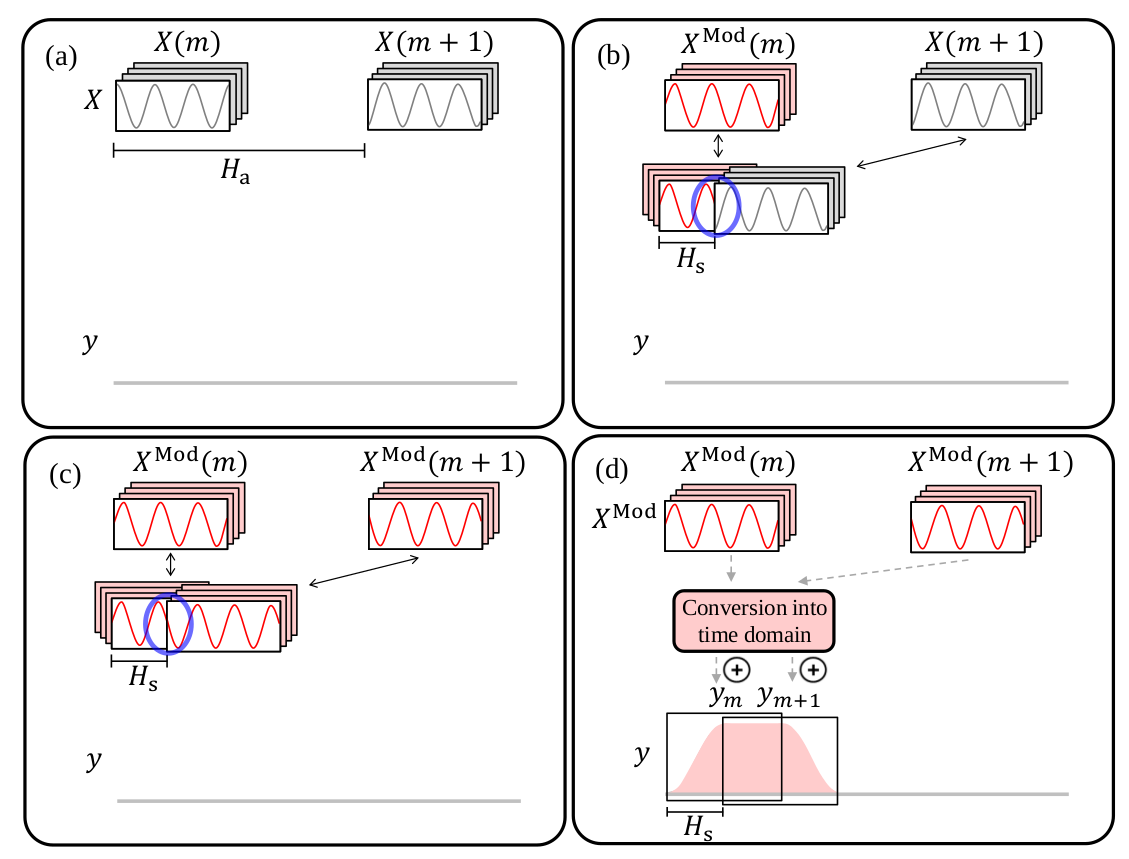
\includegraphics[width=9cm]{res/phasevocoder.png}}
    \caption{\label{fig:phasevocoder}
      Fonctionnement du vocodeur de phases [\cite{TSMreview}]. (a) Les frames sont décomposés par le STFT. (b) Les phases des 2 frames sont clairement pas les mêmes si on les overlap sans les manipuler. (c) La phase des frames sont propagées pour avoir une correspondence. (d) ISTFT pour reconstruire le signal après avoir fait l'overlap des frames modifiés.}
  \end{figure}

\section{Méthode développée}


Le live-coding (aussi nommée \emph{programmation à la volée}) est une technique de programmation de
façon improvisée afin d'avoir des résultats artistiques. Il existe plusieurs domaines dans lesquels
le live coding s'applique, comme la génération de graphismes ou de la musique. Évidement, dans cet
article l'approche musicale du live-coding a été exploitée pour pouvoir implémenter un algorithme
de time stretching en temps réel.

J'ai implementé un granulateur qui utilise la méthode OLA basique. Pour faire cela j'ai utilisé la
librairie \emph{Overtone} en Clojure qui est utilisée pour faire de la synthèse de son en temps
réel et du live-coding en base de \emph{SuperCollider} [\cite{SonicPI}].

\paragraph {Overtone}

Clojure est un langage fonctionnel qui a plusieures caractéristiques intéressantes dans notre sujet.
Premièrement,en étant un langage fonctionnel hérité de Lisp, donc toutes les données sont manipuléss
de façon mathématique avec des fonctions [\cite{Clojure}].\\
Deuxièmement, Clojure utilise le interpreteur de ligne de comande \emph{Leiningen}, qui permet
d'exécuter des commandes en temps réel tapées par l'utilisateur.

\begin{figure}[h]
    \centerline{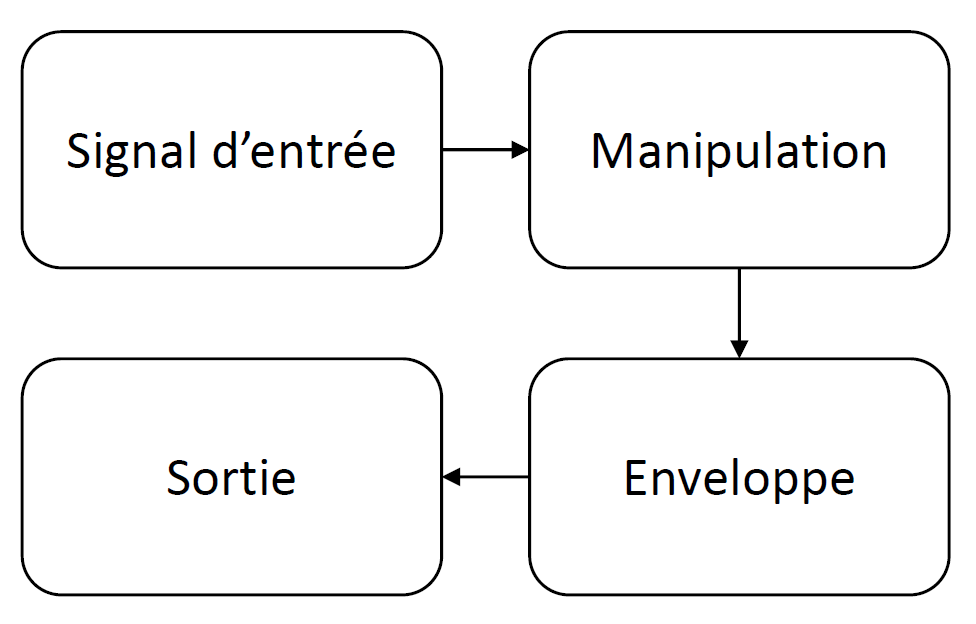
\includegraphics[width=9cm]{res/synthetiseur.png}}
    \caption{\label{fig:synthetiseur}
      Fonctionnement d'un synthétiseur [\cite{TSMreview}].
      Le fonctionnement d'un synthétiseur se résume en une ``boîte noire'' qui prend
      un signal, le manipule (filtres, enveloppe, etc...) et ensuite fait un output.
      Plusieures manipulations peuvent être imbriquées.
    }
  \end{figure}

  D'un autre coté, SuperCollider est un environnement et un langage de programmation pour faire
  de la synthèse en temps réel. SuperCollider fonctione basiquement avec des ``synth'' (synthétiseur)
  qui prennent un signal (que ce soit une onde ou un buffer avec des segments temporels de son),
  les manipule et puis les renvoit.
  
  Ces manipulations sont faites avec des UGens (Unit Generator) qui sont des blocs pour
  analyser/synthétiser des sons (par exemple, un filtre passe bas, un oscilateur sinusoïdale,
  un ugen pour lire un buffer, etc...). Les résultats d'un UGen peuvent être passés à un autre UGen
  qui peut faire d'autres manipulations (voir Figure \ref{fig:synthetiseur}).
  Aussi, les paramètres des ``synth'' sont modifiables en temps réel. C'est à dire, lorsque cet
  instrument est en train de jouer, nous pouvons changer, par exemple, la modulation d'un filtre
  et faire qu'il sonne différement lorsqu'il est lu par le serveur.
  
  Overtone profite du langage fonctionnel et les capacités de synthèse de SuperCollider pour faire
  une liaison entre les 2, le fonctionnement des langages fonctionnels se ressemblant fortement
  au fonctionnement des synthétiseurs.

  \paragraph {Granulateur}
  Le granulateur, comme son nom indique, est un synthétiseur qui manipule des grains comme on les a vu
  précédement. Ce granulateur peut servir à implémenter beaucoup d'algorithmes avec des grains, mais
  dans ce cas là nous allons l'utiliser pour implémenter un  algorithme OLA asynchrone.

  Dans cette approche, le granulateur se compose d'un \emph{scheduler} et d'un
  générateur de grains [\cite{RealTimeGrainsTSM}].\\
  Le \emph{scheduler} s'occupe de lancer le bon grain au bon moment à la sortie grâce à des paramètres
  pour définir le type de grain et à quelle vitesse les lancer. Dès qu'il veut lancer un grain, il
  va génerer le grain dont on a besoin grâce au générateur de grains.

  Pour ceci on va gérer 4 paramètres.
  \begin{itemize}
  \item \textbf{Le rate}
  \item \textbf{La durée d'un grain}
  \item \textbf{Le délai entre 2 grains}
  \end{itemize}

  Le fonctionnement de ce granulateur peut se résumer dans le pseudocode suivant:
\begin{algorithm}                      % enter the algorithm environment
\caption{Scheduler du granulator}      % give the algorithm a caption
\label{alg:granulator}                 % and a label for \ref{} commands later in the document
\begin{algorithmic}                    % enter the algorithmic environment

\STATE scale $\Leftarrow$ le ratio  
\STATE duration $\Leftarrow$ durée d'un grain
\STATE delay $\Leftarrow$ délai entre grains grain 
\STATE phasor $\Leftarrow$ pointeur dynamique qui avance au rythme du scale
\STATE last $\Leftarrow$ le moment où le dernier grain a été lancé
\STATE time $\Leftarrow$ le temps courant
\STATE N $\Leftarrow$ la taille du morceau analysé
\STATE last $=$ time

\WHILE{$phasor<N$}

\IF{time $\leq$ last + delay$*$duration}
\STATE generateGrain(phasor, duration)
\STATE last $=$ time
\ENDIF
\STATE phasor $=$ update(phasor)
\STATE time $=$ update(time)
\ENDWHILE
  \end{algorithmic}
\end{algorithm}

Le phaseur est un pointeur dynamique qui va parcourir le fichier à lire à la vitesse du ratio passé
en paramètre. Les fonctions update du pseudocode vont mettre a jour ces variables (par rapport au
temps). La méthode generateGrain prend en paramètre un indice et la durée, donc cette méthode va
renvoyer un grain qui commence à $phasor$ et qui finit à $phasor+duration$.

\paragraph{Implementation}
Ce granulateur a été implémenté en Overtone (voir Annexe pour code source) en définissant
un ``synth'' (méthode defsynth), et pour créer ce synth on a utilisé les UGen suivants.
L'UGen \verb+trig1+ est un fonction qui va activer l'ugen auquel on va lui associer, il
prend une onde en paramètre (dans notre cas, un \verb+sin-osc+), il va server de \emph{scheduler}.
Puis nous avons un \verb+phasor+ qui va parcourir le fichier à la vitesse définie par notre paramètre
de ratio. On a donc associé notre trigger à un UGen \verb+env-gen+ qui va créer un grain grâce à
une enveloppe basée sur la fenêtre de Hanning. Finalement un UGen \verb+play-buf+ va jouer le grain
qui sera trig à la position du \verb+phasor+.

Grâce au fait que ça a été défini dans un synth, les paramètres peuvent être modifiables lors de son
exécution, nous donnant aussi la possibilité de le modifier en temps réel tel un VST ou ``plugin''
[\cite{VST}].

\paragraph {MIDI}

\begin{figure}[h]
    \centerline{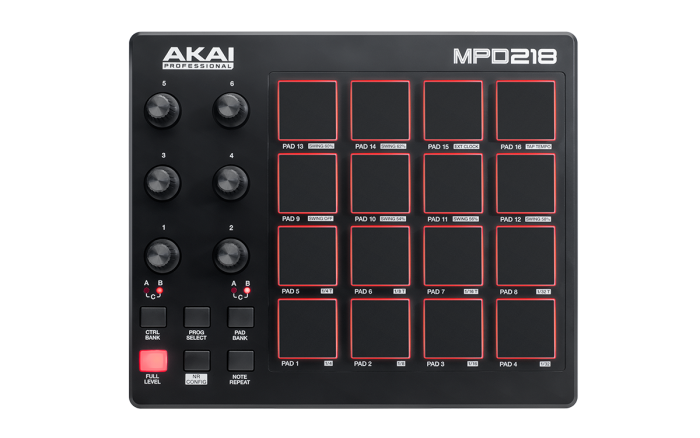
\includegraphics[width=9cm]{res/mpd218.png}}
    \caption{\label{fig:mpd218}
      Instrument MIDI (Akai MPD218). Cet instrument a été utilisé pour
      changer les paramètres du granulateur en temps réel.
    }
  \end{figure}

À continuer demain
\section{Résultats}

% [ À FAIRE TABLEAU COMPARATIF DE STYLES]

On va analyser les morceaux musicaux de différents styles et les paramètres qu'on a du utiliser
pour 


\section{Remerciements}
  Je remercie mon prometeur, Bernard Fortz, de m'avoir fait découvrir
  les yeux au monde du live-coding et la programmation fonctionnelle.

  Je tiens aussi à remercier l'UrLab pour m'avoir accueilli au SmartMonday
  pour partager avec eux tout ce que j'ai appris lors de mes recherches
  pour ce mémoire.

  Je voudrais aussi remercier mon collègue Antoine Passemiers pour m'avoir donné autant de conseils
  lors de la réalisation de ce mémoire.

  Et pour finir je voudrais remercier à Sam Aaaron pour tout son travail dans le domaine du live-coding
  et de la pédagogie avec Overtone et Sonic Pi.

\footnotesize

\bibliographystyle{apalike}
\bibliography{rapport}


\begin{appendices}
  \section{Démonstrations}
  Lien vers une vidéo démonstration de l'usage du granulateur avec le MPD218: 
  \url{https://twitter.com/Abdulitokun/status/866394006917451777}

  Le code source, ainsi que le rapport se trouvent dans le lien suivant:
  \url{https://github.com/Abde-/info-f-308mem}

  
\end{appendices}

\end{document}
